\subsection{Introducción}
Este es un ejemplo de cómo incluir una figura, una tabla y citas bibliográficas en el reporte.

\subsubsection{Ejemplo de Citas Bibliográficas}
A continuación se muestran ejemplos de diferentes tipos de referencias: un artículo \cite{chen2022new}, una tesis doctoral \cite{schelin2012spatial}, un libro \cite{konstantin2013unequal}, un documento misceláneo \cite{balestrini2018map}, un capítulo de libro \cite{delmelle2012spatial} y normas \cite{UNE77270, NCH3387}.

\subsubsection{Ejemplo de Figura}
A continuación se presenta una figura de ejemplo (véase \refer{Figura}{fig:ejemplo}).

\begin{figure}[H]
    \centering
    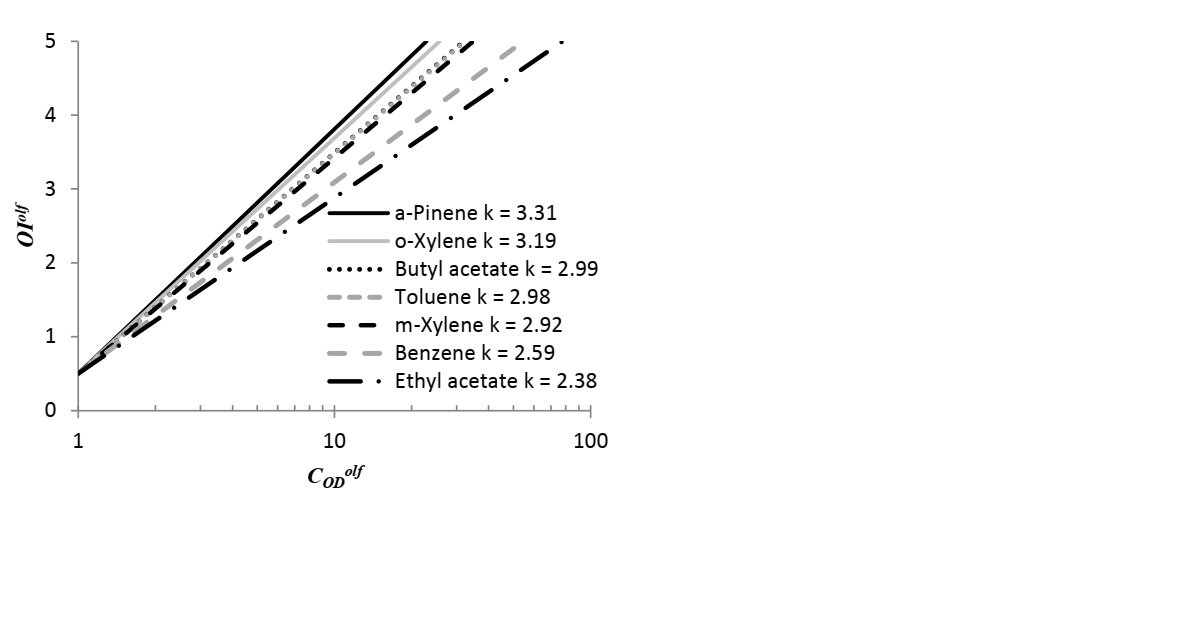
\includegraphics[width=0.8\textwidth]{Fig1.jpg}
    \caption{Descripción de la figura de ejemplo.}
    \label{fig:ejemplo}
\end{figure}

\subsubsection{Ejemplo de Tabla}
En la \refer{Tabla}{tab:ejemplo} se muestran los datos cargados desde un archivo CSV.

\begin{table}[H]
    \centering
    \caption{Datos de ejemplo cargados desde CSV.}
    \label{tab:ejemplo}
    \begin{adjustbox}{max width=\textwidth}
        \csvautotabular{tables/table.csv}
    \end{adjustbox}
\end{table}

CONTENIDO ADICIONAL DEL CAPÍTULO
